\begin{figure}[H]
\centering

\begin{subfigure}{0.48\textwidth}
\centering
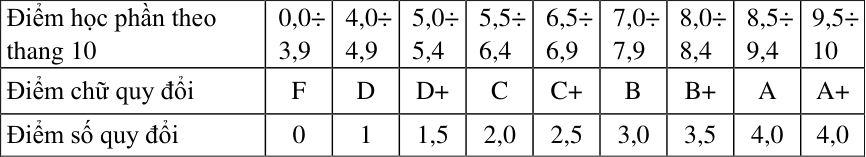
\includegraphics[width=\linewidth]{figures/table_original.png}
\caption{Bảng gốc}
\end{subfigure}
\hfill
\begin{subfigure}{0.48\textwidth}
\centering
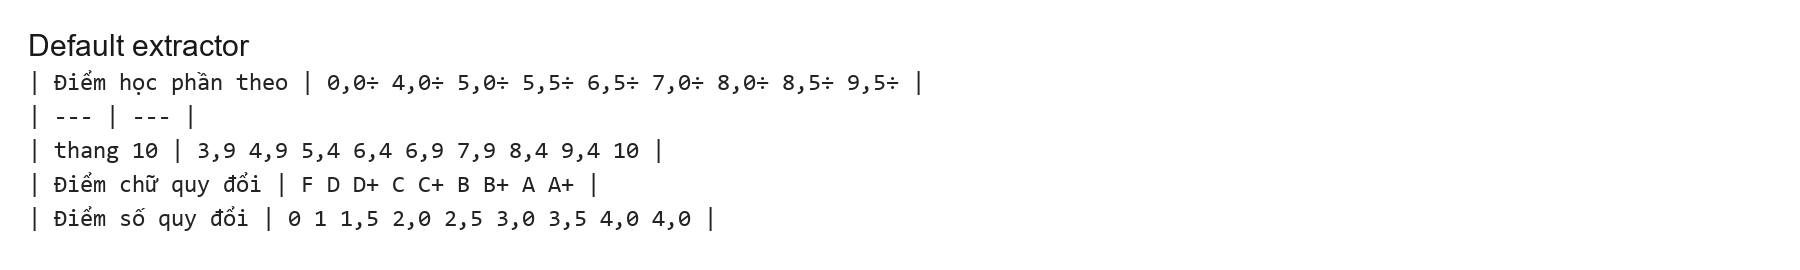
\includegraphics[width=\linewidth]{figures/table_default_output.png}
\caption{Default extractor}
\end{subfigure}

\vspace{0.25cm}

\begin{subfigure}{0.48\textwidth}
\centering
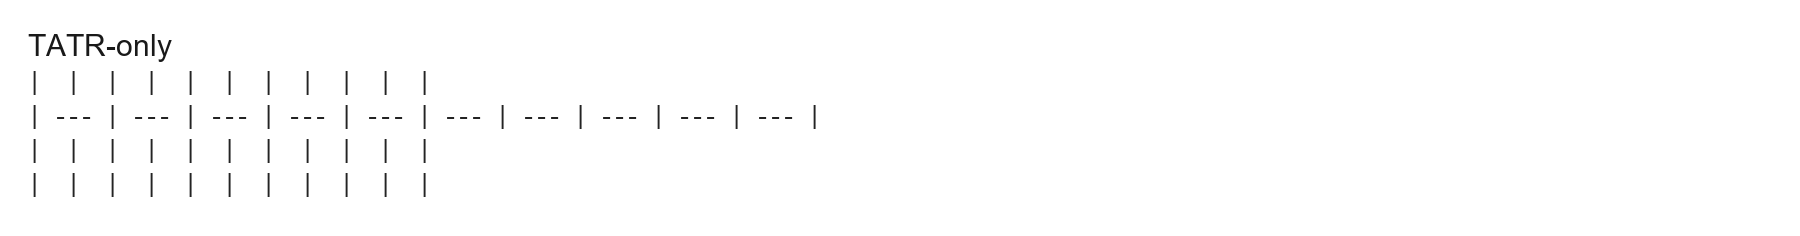
\includegraphics[width=\linewidth]{figures/table_tatr_output.png}
\caption{TATR-only}
\end{subfigure}
\hfill
\begin{subfigure}{0.48\textwidth}
\centering
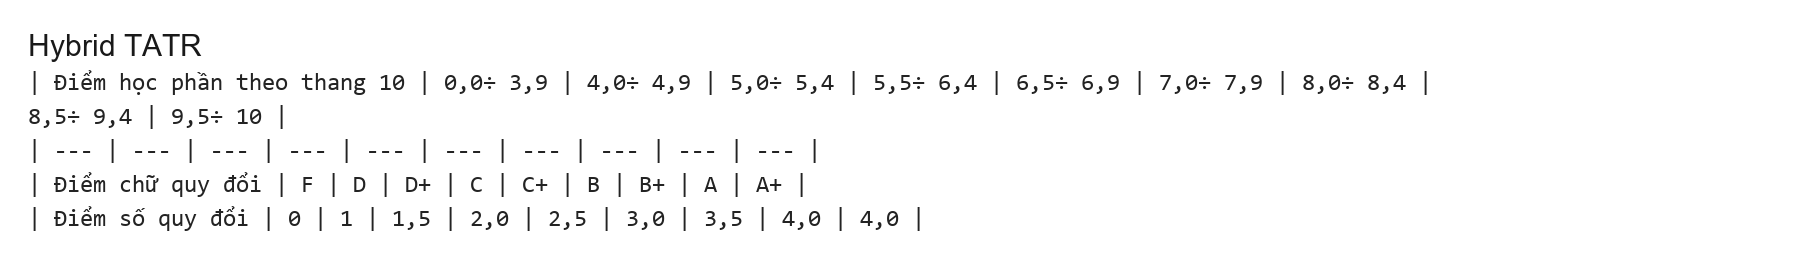
\includegraphics[width=\linewidth]{figures/table_hybrid_tatr_output.png}
\caption{Hybrid TATR}
\end{subfigure}

\caption{Minh họa đầu ra của các backend trích xuất bảng trên cùng một bảng QCDT trang 9}
\label{fig:qcdt-page9-table-backend-visual-output}
\end{figure}
